\section{Durchführung}
\label{sec:Durchführung}
\subsection{Einseitige Einspannung}
Der Stab wird in der Apperatur wie in Abb. \ref{fig:apperatur} eingespannt.
Die Stäbe wurden schon häufiger gebogen und sind in der Ruheposition nicht mehr exakt gerade.
Daher wird zuerst die Durchbiegung des Stabes ohne Last $D_0(x)$ mithilfe der Messuhren vermessen.
Im Anschluss wird ein Gewicht $F$ am Ende des Stabes befestigt, so dass eine Auslenkung von $\SI{3}{\mm} - \SI{7}{\mm}$ erreicht wird.
Nun wird die Durchbiegung mit Masse $D_\text{M}(x)$ gemessen.
Die reale Durchbiegung beträgt dann
\begin{equation}
    D(x) = D_\text{M}(x) - D_0(x) .
    \label{eqb:D_real}
\end{equation}

\begin{figure}
    \centering
    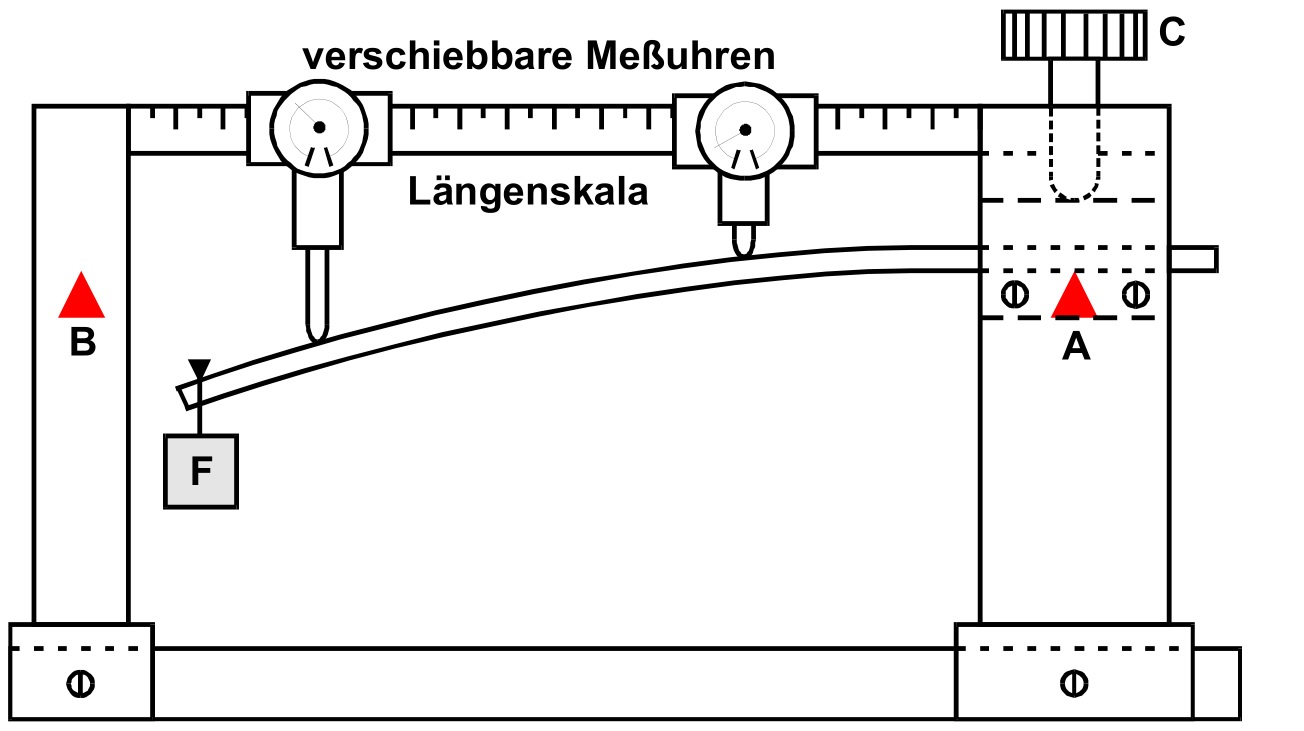
\includegraphics[width=0.5\textwidth]{content/data/apperatur.jpg}
    \caption{Darstellung der Apperatur zur einseitigen Biegung eines Stabes. \cite{anleitung}}
    \label{fig:apperatur}
\end{figure}

\subsection{Zweiseitige Biegung}
